\chapter{Manual de usuario y casos de uso}
\label{cap:Capítulo 5}
En este capítulo realizaremos un recorrido guiado sobre el uso de nuestra aplicación, así como los requisitos que el usuario tiene que tener instalados antes de poder utilizarla. Explicaremos paso a paso los programas que nosotros hemos utilizado, mencionando posibles alternativas que podrían sustituirlos, así como todas las opciones que hay a disposición del usuario en la parte de la aplicación, adjuntando también capturas de pantalla de cada una de las acciones a realizar.

\section{Guía para la instalación}

En este apartado explicamos los requisitos previos de la aplicación, es muy recomendable que esta instalación se lleve a cabo por una persona con conocimientos informáticos, ya que puede ser un poco compleja para una persona que no tenga una base en cuanto al uso de Python o la línea de comandos.
Vamos a enumerar las herramientas, tecnologías y librerías necesarias para poder correr la aplicación en local. Vamos a enumerar las que nosotros hemos utilizado, pero cualquier aplicación con su misma funcionalidad podría servir En primer lugar debes instalarte el servidor local  \textbf{Xampp} para que la aplicación pueda conectarse con la base de datos. A continuación debes instalar la herramienta \textbf{Visual Studio Code} con la que correrás nuestro código. Una vez te la hayas instalado debes descargarte el \textbf{intérprete} anaconda para poder instalar las siguientes librerías Python con estos comandos:
\begin{itemize}
	\item pip install tk
	\item pip install sqlite
	\item pip install selenium
	\item pip install googletrans
	\item pip install text2emotion
	\item pip install zipfile38
	\item pip install inspect-it
	\item pip install python-time
	\item pip install pytest-shutil
	\item pip install stats
	\item pip install mysql-connector-python
	\item pip install jsonlib
	\item pip install webbrowser
	\item pip3 install jicson
	\item pip install python-csv
\end{itemize}
Una vez realizadas estas instalaciones para la parte del back-end, debes instalarte \textbf{node.js} para el front-end, y una vez lo tengas( lo cual te permitira usar npm para instalar componentes react), buscar en la barra de Windows la consola powerShell para instalar los siguientes componentes de React:
\begin{itemize}
	\item npm install
	\item npm i -S react-router-dom
	\item npm i -S react-router
	\item npm i -S react-photo-gallery
	\item npm i -S react-images
	\item npm i -S simple-react-google-maps
	\item npm i -S react-circle-modal
	\item npm i -S react-vertical-timeline-component
	\item npm i -S rsuite-table
	\item npm i -S react-awesome-button
	\item yarn add react-router-dom
	\item yarn add react-router
	\item react-photo-gallery
	\item yarn add react-images
	\item yarn add simple-react-google-maps
	\item yarn add react-circle-modal
	\item yarn add react-vertical-timeline-component
	\item yarn add rsuite-table
	\item yarn add react-awesome-button
\end{itemize}

 Una vez tengas todo esto instalado debes arrancar Visual Studio Code e importar el proyecto o descargarlo de nuestro Github, para ello, una vez lo tengas en local, selecciona ``abrir'', ``Proyecto existente'' y busca en tu explorador de archivos el proyecto. Después selecciona el archivo master.py y ejecuta el código con Python o python3 (el botón de play verde, si usas VScode). Te saltará una ventana, pero todavía tienes que abrir otros archivos. Después, hemos proporcionado un archivo para PoweShell que ejecuta la aplicación en yarn, el cual se llama ``powershell.ps1'' solo tienes que ejecutarlo como administrador y él hará el resto, también puedes iniciar yarn directamente desde la consola. Por último, para tratar los datos, deber iniciar los apartados de Apache y MySQL de Xampp, para que se puedan tratar los datos. Con esto ya estaría todo listo para que empieces a trabajar con nuestra aplicación siguiendo el manual de usuario.
 
 Recuerda tener disponible también un navegador web, recomendablemente Google Chrome, para poder descargar los datos de las redes objetivo y posteriormente correr la aplicación web y visualizar los datos.

\section{Manual de usuario}
 
En este apartado vamos a ver cuál es la forma de utilizar la aplicación una vez instaladas todas las dependencias, la cual consta de cuatro fases diferenciadas, el login en la aplicación de escritorio, la descarga de los datos de Facebook y Google, el tratamiento de los datos por parte de nuestro programa y por último la visualización de los mismos a través de la interfaz web. A continuación los explicaremos en más detalle:

\subsection{Bienvenida y login}
Esta es la primera ventana con la que se encuentra el usuario, consta de tres botones, uno de descarga, donde el usuario se va a registrar y descargar sus datos para que podamos tratarlos, otro de creación de las bases de datos, así como la visualización de los mismos y un último botón para salir de la aplicación:
 \begin{figure}
 	\begin{center}
 		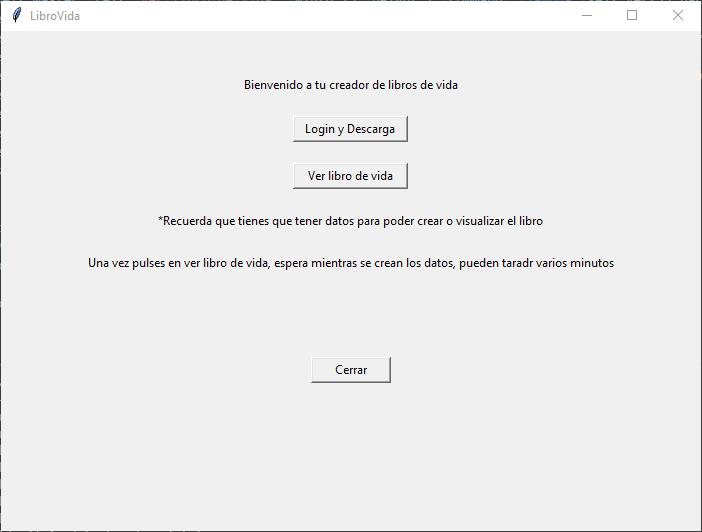
\includegraphics[scale=0.7]{Imagenes/Fuentes/PantallaPrincipalOpciones.png} 
 		\caption{Inicio de sesión}
 		\label{PantallaPrincipalOpciones}
 	\end{center}
 \end{figure}
 
 Si intentas crear datos o visualizarlos antes de tenerlos descargados, la aplicación es posible que falle, por lo que si no tienes las carpetas de datos (Carpeta\_G y Carpeta\_FB) ya creadas, lo primero va a ser la descarga. Para ello, el botón de  ``Login y descarga'' te lleva a la pestaña donde comprobamos si ya te has descargado los datos, donde se descargaran primeramente los de Facebook y después pasaremos a los de Google: 
 
 \begin{figure}
	\begin{center}
		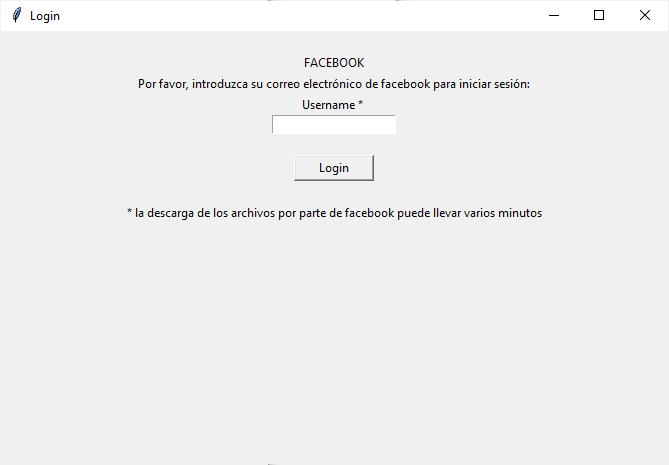
\includegraphics[scale=0.7]{Imagenes/Fuentes/PantallaLogin.png} 
		\caption{Login para descarga}
		\label{PantallaLogin}
	\end{center}
\end{figure}

\subsection{Descarga de Datos}

Esta parte esta comandada por Selenium, una aplicación que, manejando una ventana de Google Chrome, para ayudarte a descargar los datos de Facebook. Esta ventana se abrirá directamente en la página de Login de Facebook, en al que te tendrás que registrar, Selenium ya te facilita el mismo correo que has añadido en el registro de la aplicación para ahorrarte tiempo. Este Login se puede ver en la figura 5.1 

\begin{figure}
	\begin{center}
		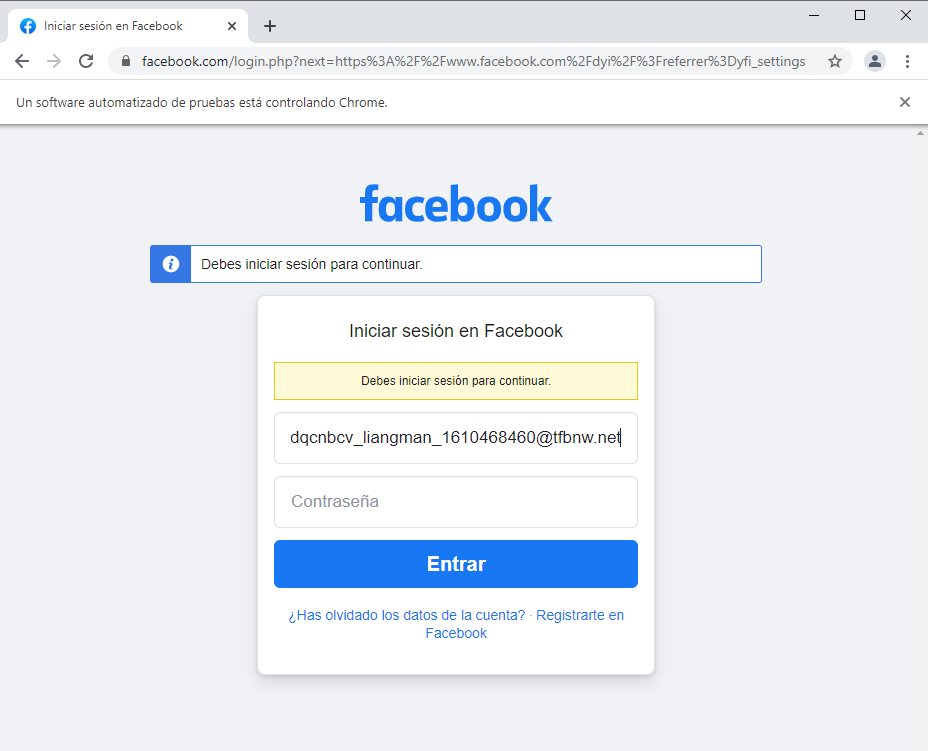
\includegraphics[scale=0.5]{Imagenes/Fuentes/TutorialDescarga1.png} \caption{Login Facebook}
		\label{TutorialDescarga1}
	\end{center}
\end{figure}


Así solo tendrás que escribir tu contraseña y Selenium te enviara directamente a la página de descarga, donde te mostrara un vistoso tutorial que te indica los pasos a seguir (Mostrados en la figura 5.2), los cuales son:

\begin{itemize}
	\item Cambiar el formato de HTML a JSON
	\item Pulsar el botón de ``Crear archivo''
	\item Esperar hasta que haya una copia disponible
	\item Pulsar en ``Copias Disponibles'' y después en ``Descargar''
\end{itemize}
\begin{figure}
	\begin{center}
		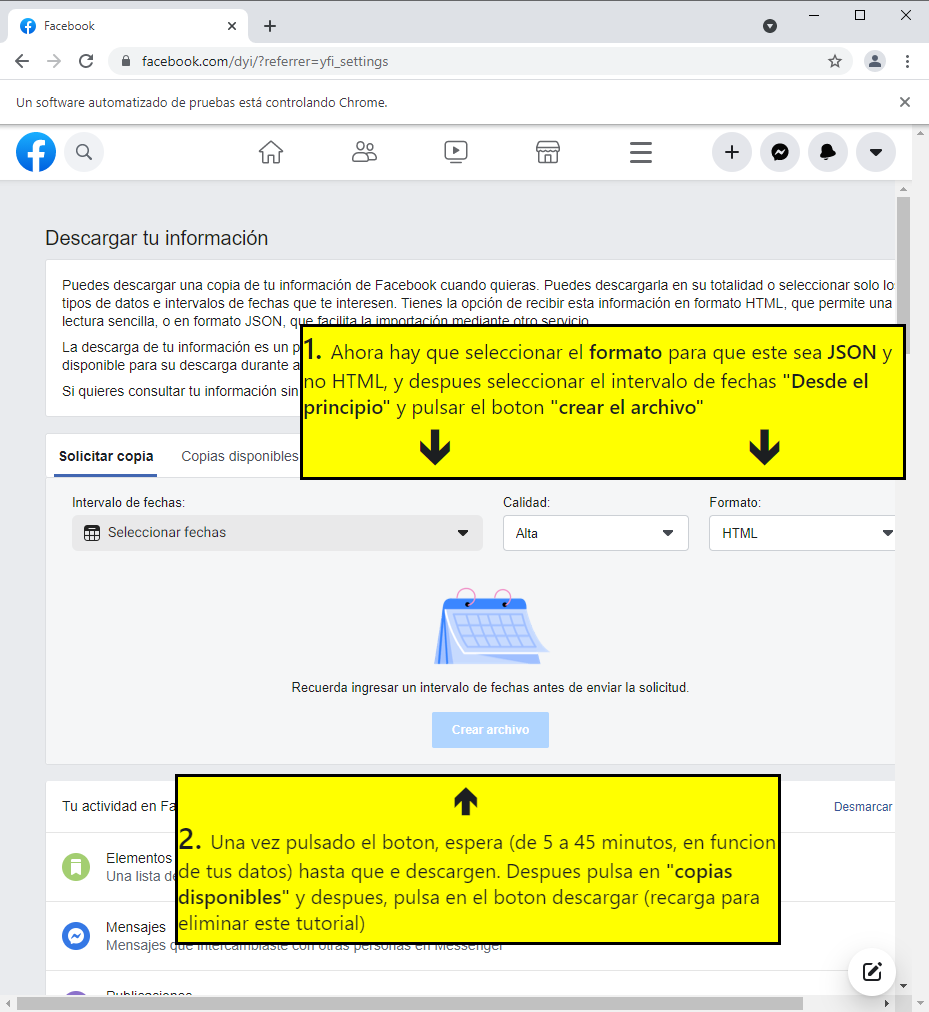
\includegraphics[scale=0.5]{Imagenes/Fuentes/TutorialDescarga2.png} \caption{página de descarga de datos}
		\label{TutorialDescarga2}
	\end{center}
\end{figure}

Una vez pulses el botón de descarga en la copia que se acaba de crear, la aplicación hará el resto. ¡No cierres la ventana! Se cerrará automáticamente.

Ten en cuenta que el tutorial puede variar, ya que Facebook esta siempre en constante cambio, si esto ocurre, te rogamos que se lo hagas saber al responsable de la aplicación.

Una vez Facebook está descargado, se te abrirá una nueva ventana de la aplicación donde se te explicara como descargar los datos de Google, en el que tendrás que pulsar ``Descargar datos Google'' si deseas que se descarguen:

\begin{figure}
	\begin{center}
		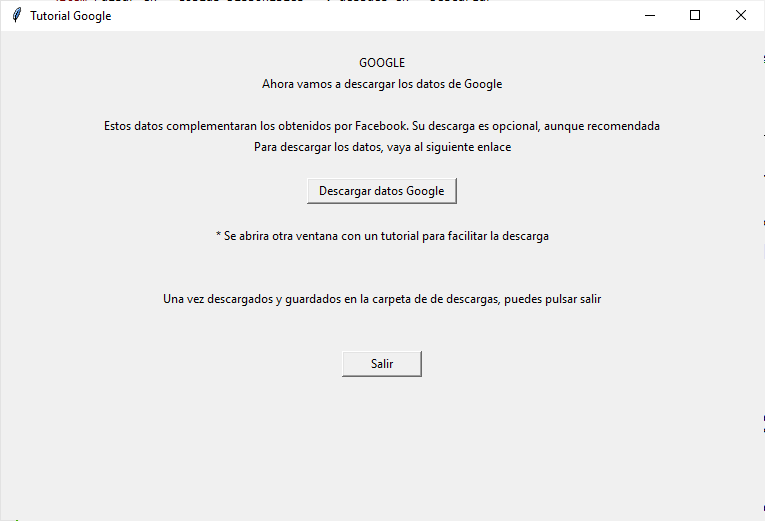
\includegraphics[scale=0.5]{Imagenes/Fuentes/TutorialDescargaG1.png} \caption{Tutorial de Google}
		\label{TutorialDescargaG1}
	\end{center}
\end{figure}

Esto debería haber abierto dos cosas, un navegador con la página de descarga y una nueva ventana de la aplicación con un tutorial donde se detalla paso a paso los requerimientos necesarios para descargarlos. Google bloquea Selenium, por lo que esta vez será el usuario que está leyendo esto el que tiene que realizar todos los pasos en la página de descarga.

A continuación mostramos algunas paginas del tutorial:
\begin{figure}
	\begin{center}
		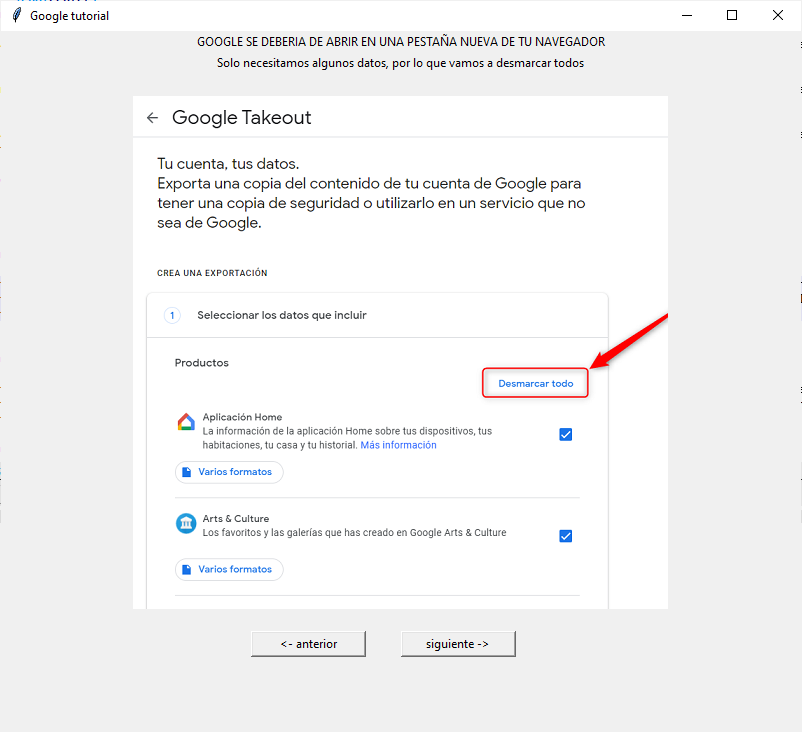
\includegraphics[scale=0.5]{Imagenes/Fuentes/TutorialDescargaG2.png} \caption{Tutorial de Google}
		\label{TutorialDescargaG2}
	\end{center}
\end{figure}
\begin{figure}
\begin{center}
	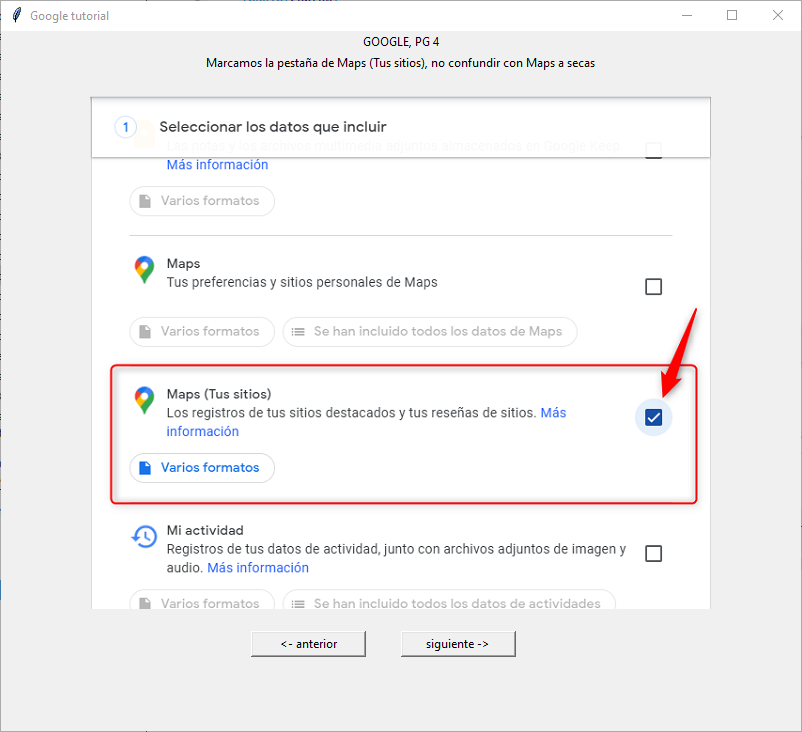
\includegraphics[scale=0.5]{Imagenes/Fuentes/TutorialDescargaG3.png} \caption{Primero desmarcamos todo}
	\label{TutorialDescargaG3}
\end{center}
\end{figure}
\begin{figure}
	\begin{center}
		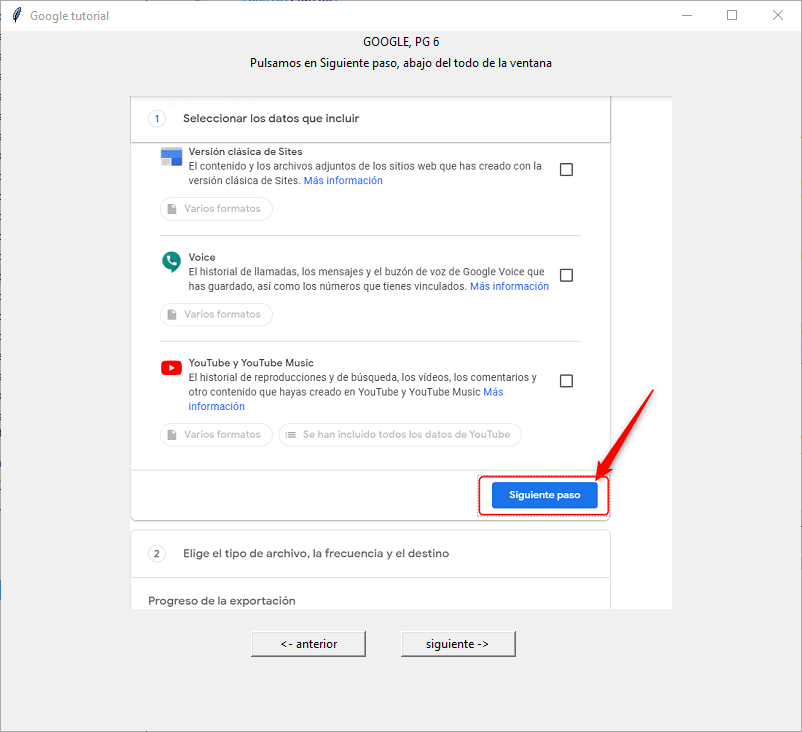
\includegraphics[scale=0.5]{Imagenes/Fuentes/TutorialDescargaG4.png} \caption{Después marcamos los datos correctos}
		\label{TutorialDescargaG4}
	\end{center}
\end{figure}
\begin{figure}
	\begin{center}
		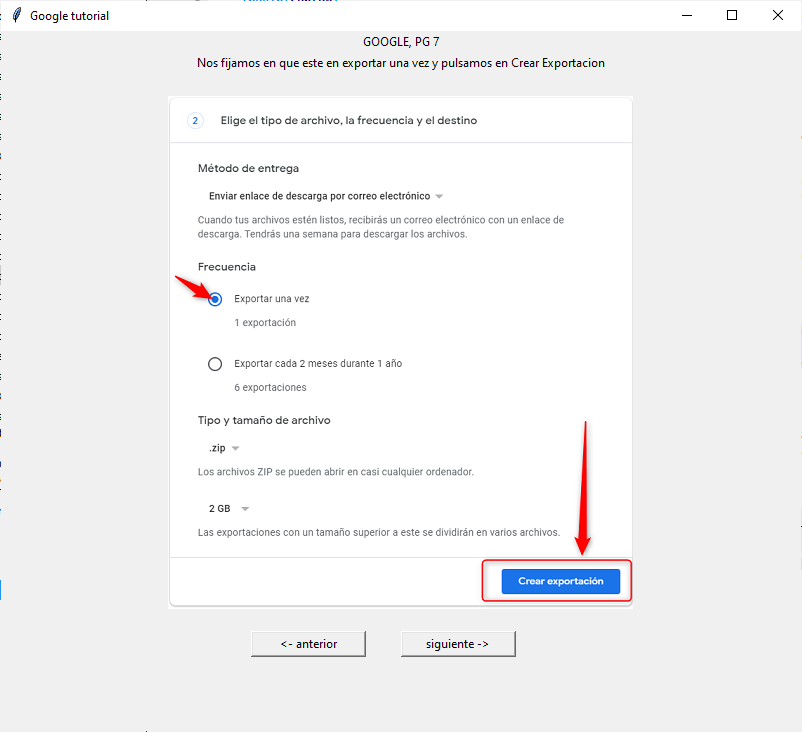
\includegraphics[scale=0.5]{Imagenes/Fuentes/TutorialDescargaG5.png} \caption{Por último nos descargamos los datos}
		\label{TutorialDescargaG5}
	\end{center}
\end{figure}

Una vez hecho esto, hay que esperar a que los datos se descarguen, tienen que estar en la carpeta de descargas, si no no se podrán analizar. Después de eso ya se puede cerrar el tutorial y tendríamos todos los datos que necesitamos descargados.

\subsection{Creación de las tablas}

Esta Sección no necesita más acción por parte del usuario que pulsar el botón de ``Ver libro de vida'' una vez los datos estén descargados, se procesara todo automáticamente y ya se podrán visualizar los datos en la interfaz. Puede Tardar un rato, así que ten paciencia.

\subsection{interfaz gráfica para visualizar datos}

A partir de la figura 5.10 vamos a mostrar la parte de la aplicación en la que más tiempo vas a pasar, es decir, la interfaz donde mostramos todos los datos una vez descargados y tratados. En las siguientes figuras iremos explicando los apartados paso a paso.

\color{blue}
La figura 5.10 muestra la parte de Home, donde presentamos el proyecto y donde se explica brevemente todo lo que se puede hacer en los diferentes apartados de la web.
\begin{figure}
	\begin{center}
		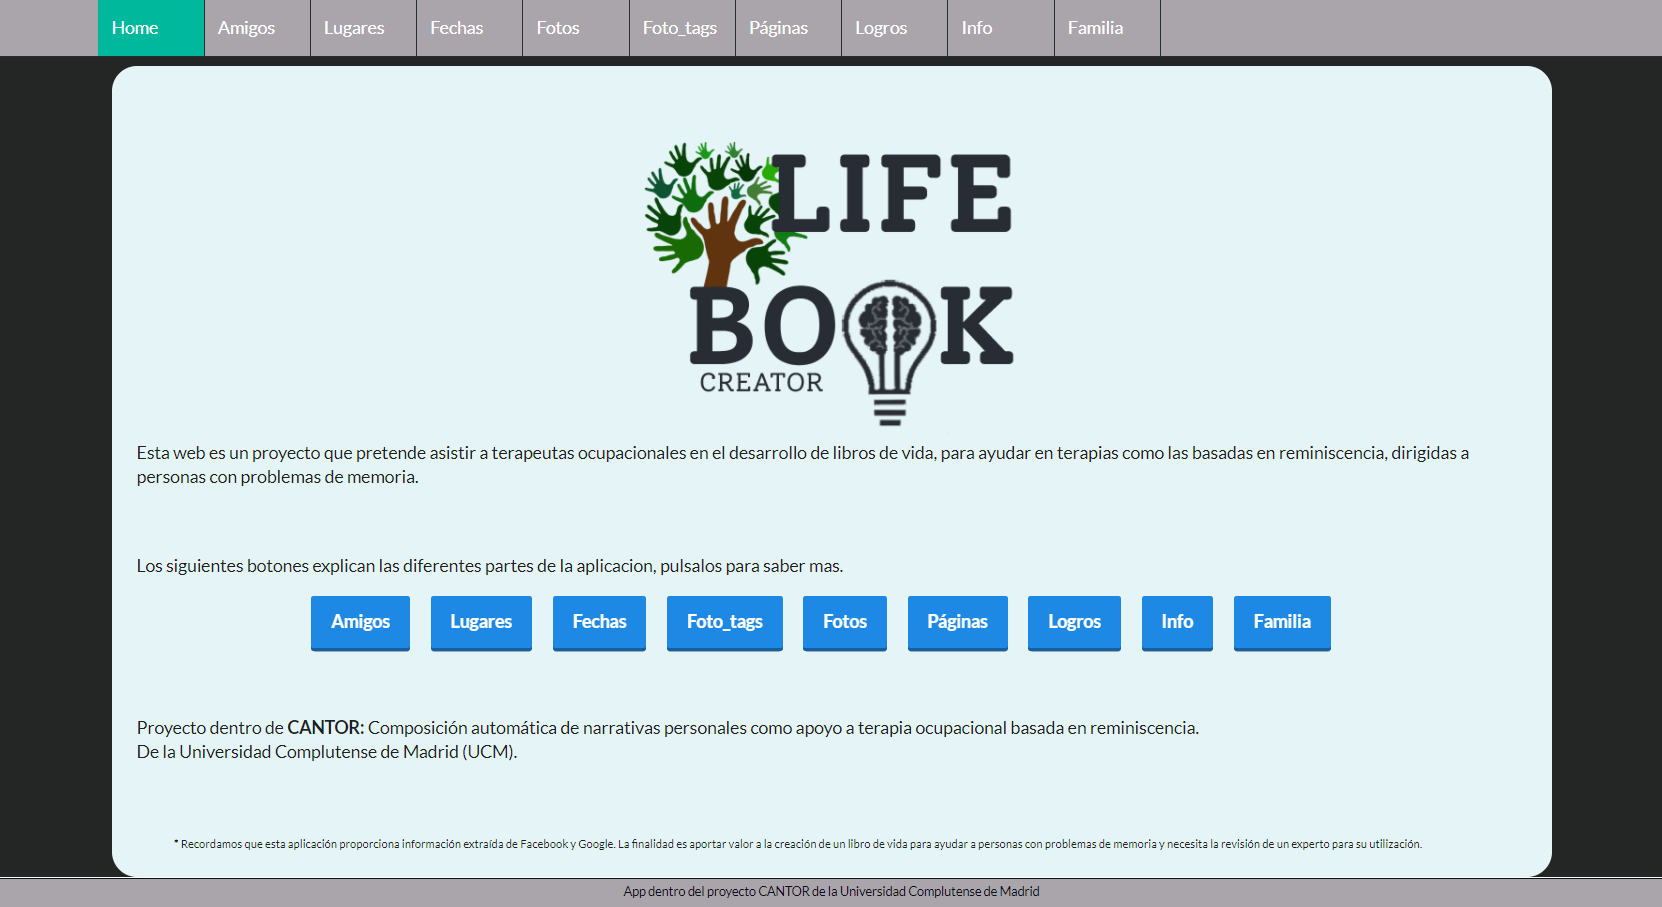
\includegraphics[scale=0.3]{Imagenes/Fuentes/InterfazHome.png} \caption{Interfaz de usuario, apartado Página principal}
		\label{WebAplication1}
	\end{center}
\end{figure}

\color{black}
En la figura 5.11 puedes ver el apartado de Amigos, en el que se muestran los diez amigos con los que más interactúas, en la figura se aprecia una tabla en la que en la primera columna se encuentra el nombre de tu amigo, seguido de la fecha en la que os hicisteis amigos en Facebook y de la puntuación obtenida basándonos en el número de veces que comentas o te comentan las publicaciones, así como las veces que reaccionáis a vuestros posts.
\begin{figure}
	\begin{center}
		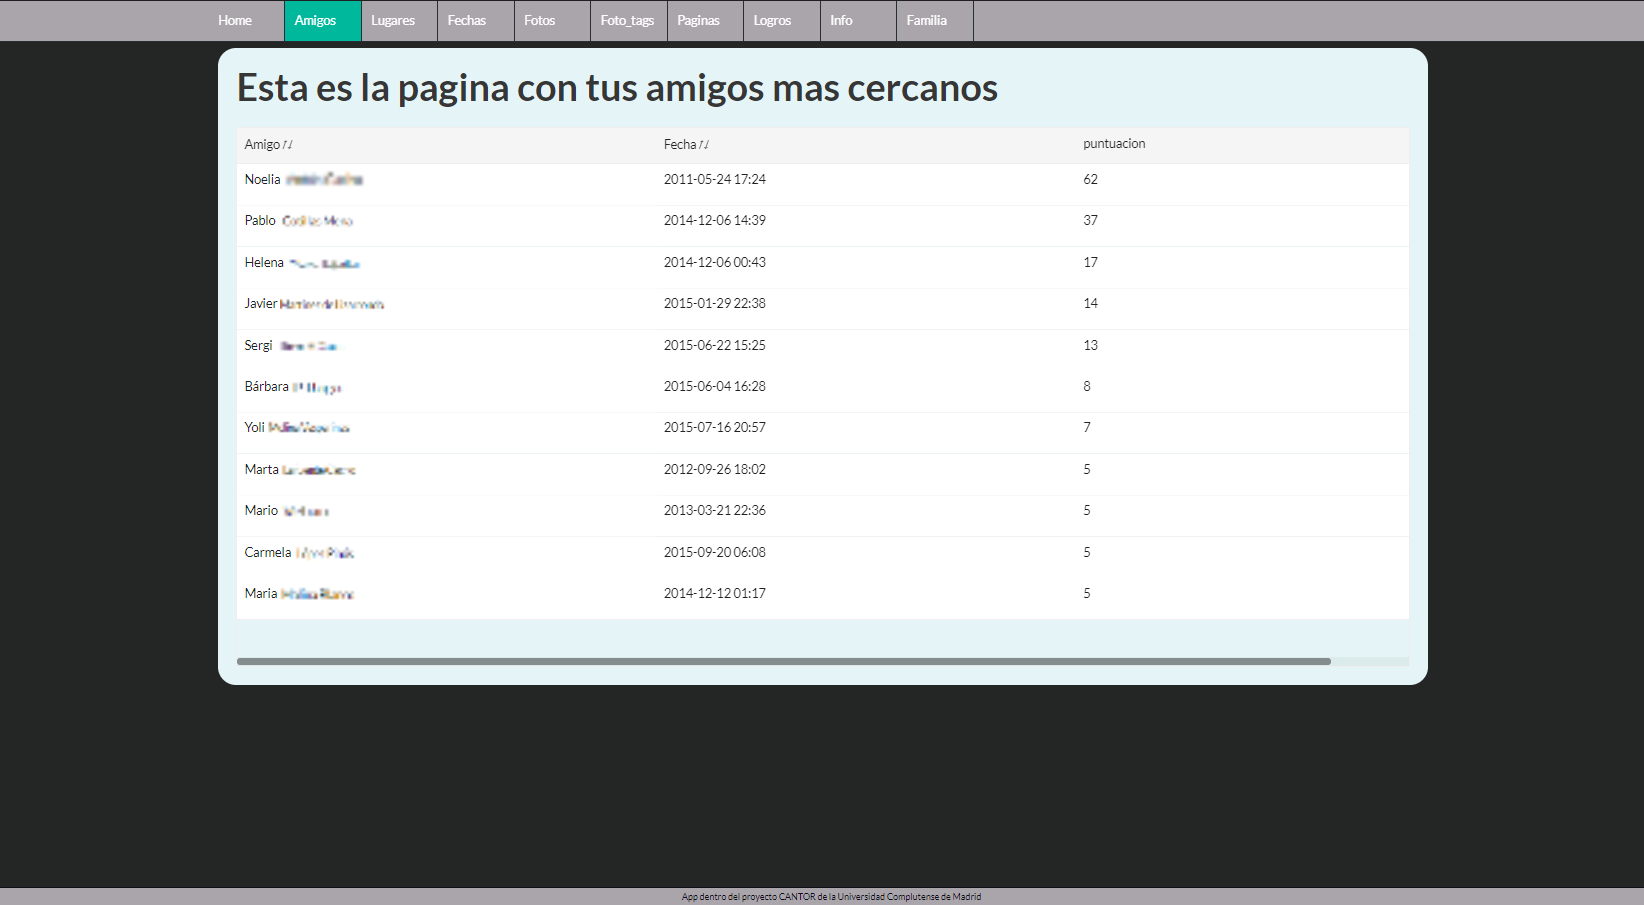
\includegraphics[scale=0.3]{Imagenes/Fuentes/InterfazAmigos.png} \caption{Interfaz de usuario, apartado amigos}
		\label{WebAplication2}
	\end{center}
\end{figure}
En la figura 5.12 y 5.13 puedes ver el apartado de Lugares, que corresponde a los distintos sitios en los que el usuario ha estado, ha publicado en Facebook o Google, así como las reseñas que ha dejado en algunos establecimientos. Se puede apreciar un mapa con marcadores que corresponde a todos esos sitios, una lista de las personas con las que ha estado, así como una galería si es que se publicó alguna foto en alguno de esos sitios.
\begin{figure}
	\begin{center}
		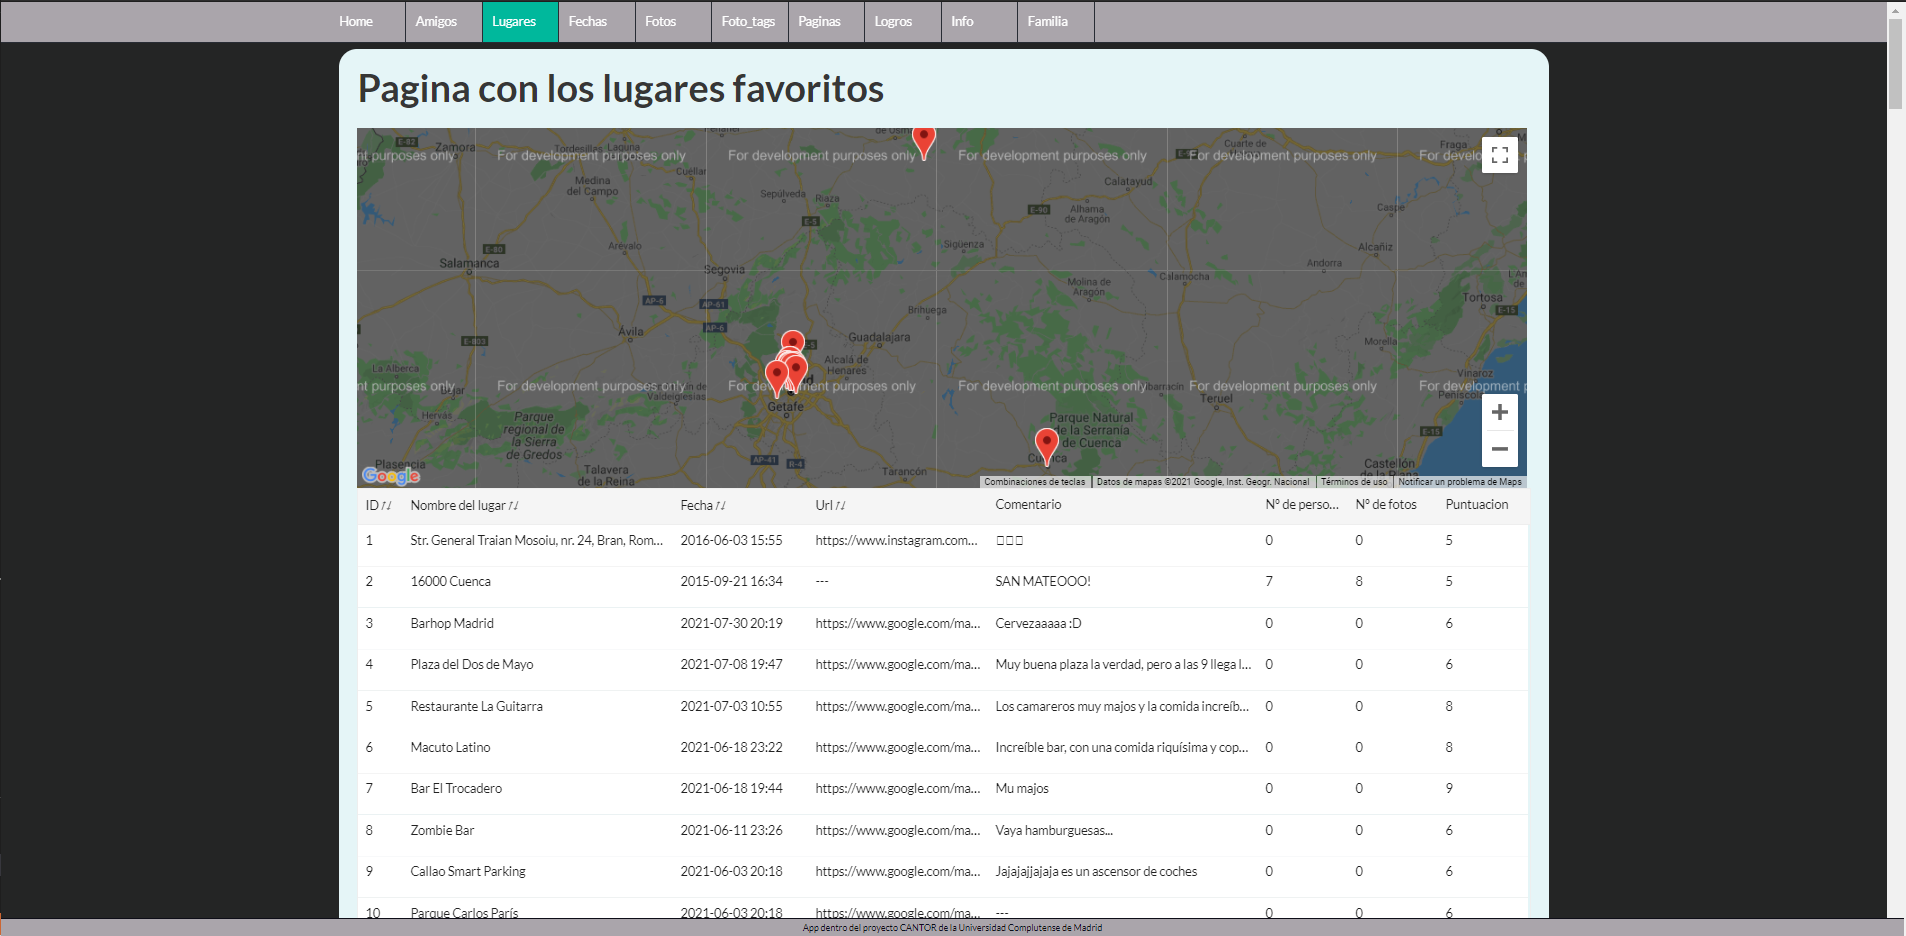
\includegraphics[scale=0.3]{Imagenes/Fuentes/InterfazLugares1.png} \caption{Interfaz de usuario, apartado lugares 1}
		\label{WebAplication3}
	\end{center}
\end{figure}
\begin{figure}
	\begin{center}
		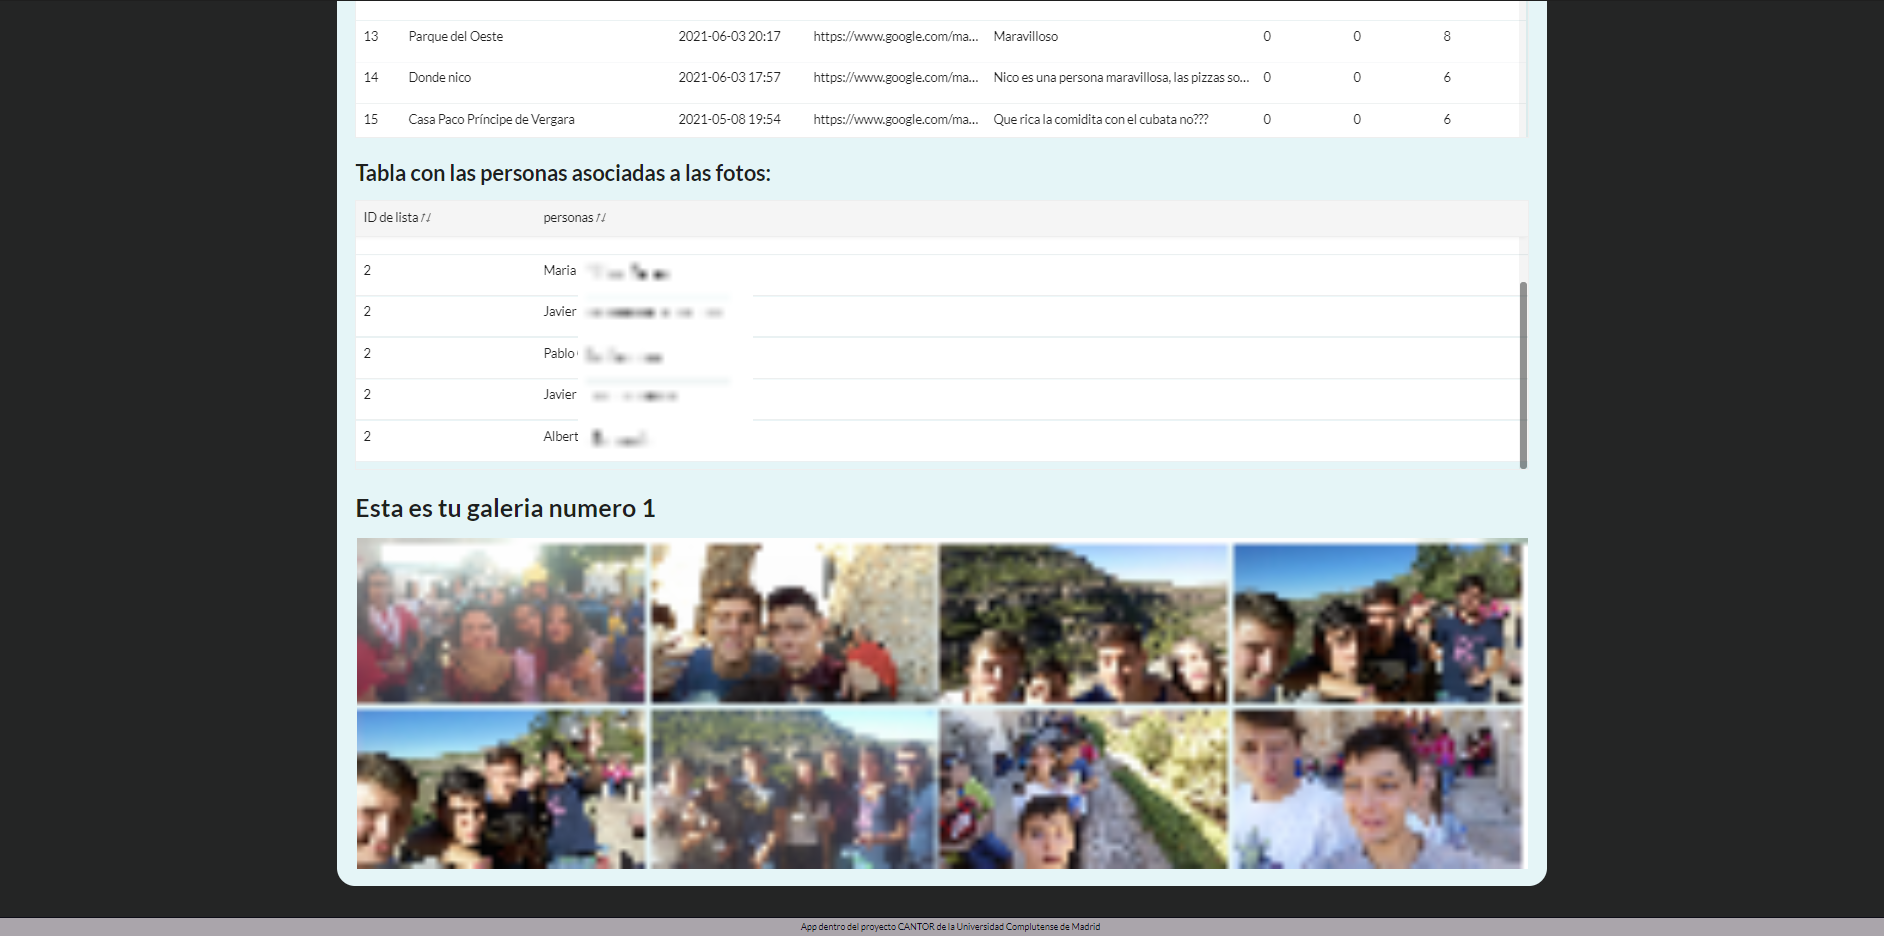
\includegraphics[scale=0.3]{Imagenes/Fuentes/InterfazLugares2.png} \caption{Interfaz de usuario, apartado lugares 2}
		\label{WebAplication4}
	\end{center}
\end{figure}
En la figura 5.14 puedes apreciar el apartado de fechas, que corresponde con una tabla de todos los datos de Facebook y Google ordenados en el tiempo, así como el suceso que tuvo lugar en esta fecha. También hay un botón que te lleva a un timeline de estas fechas.
\begin{figure}
	\begin{center}
		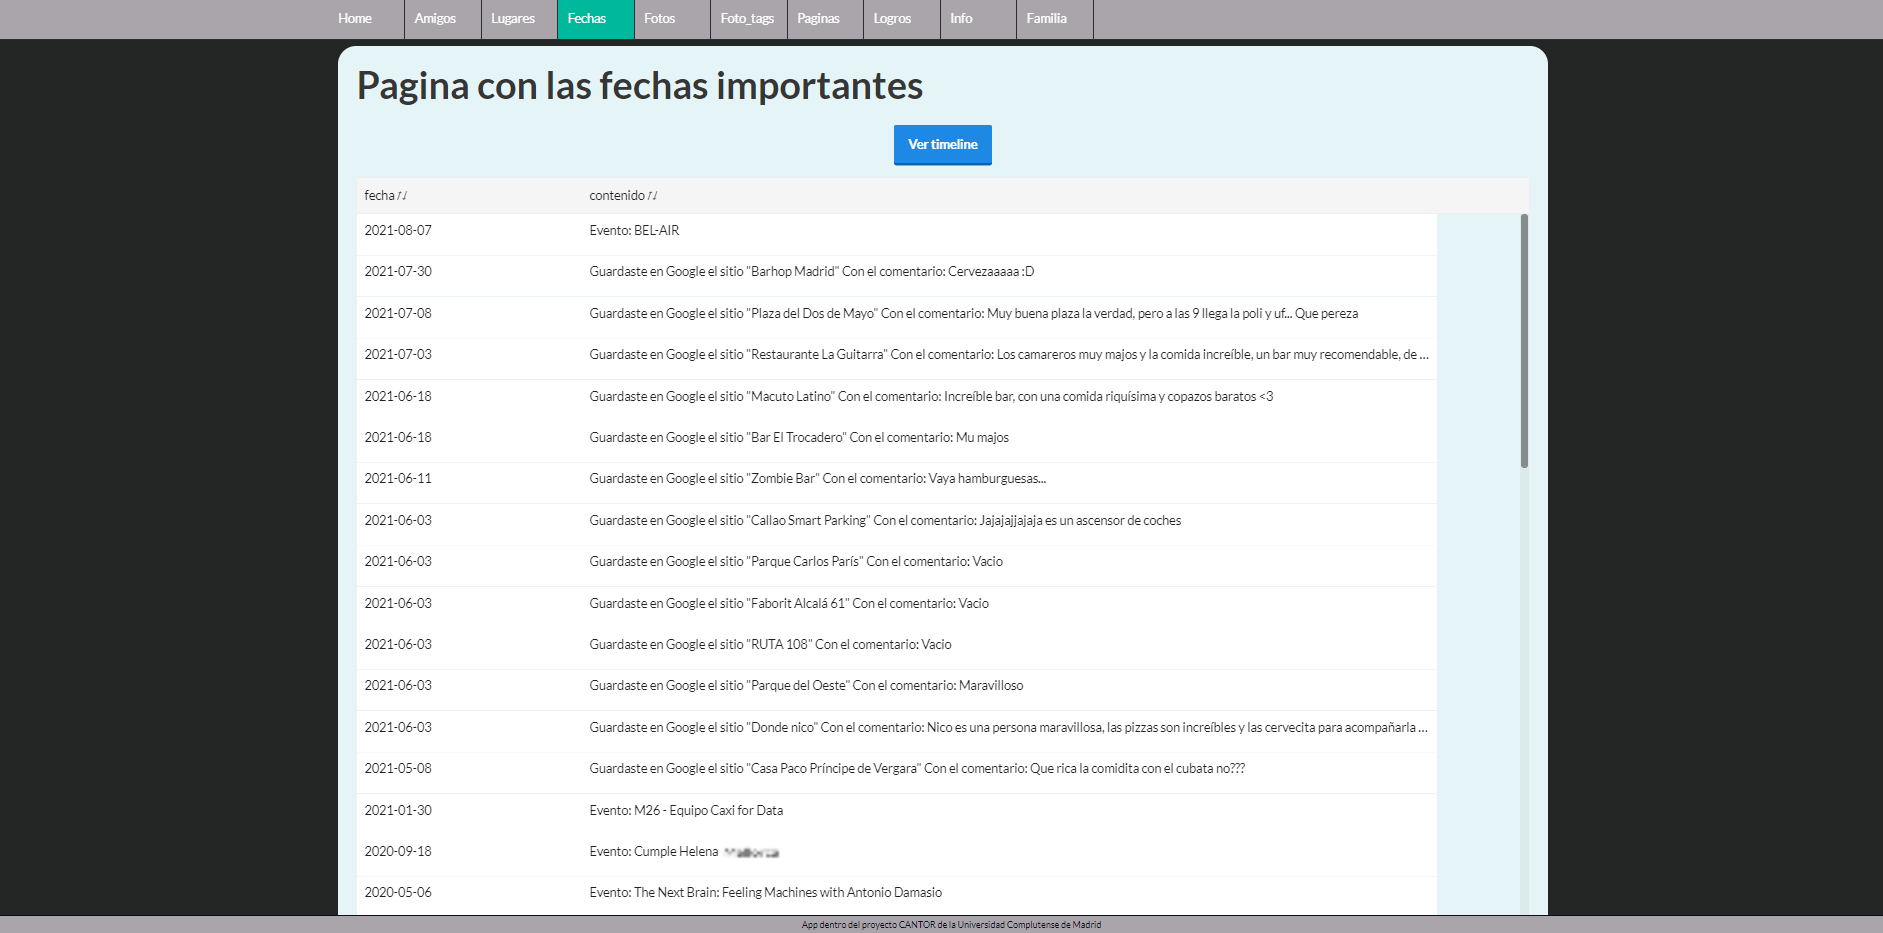
\includegraphics[scale=0.3]{Imagenes/Fuentes/InterfazFechas.png} \caption{Interfaz de usuario, apartado fechas}
		\label{WebAplication5}
	\end{center}
\end{figure}
La figura 5.15 muestra los datos de fechas que ya se han mostrado en el apartado fechas, pero de una forma más lineal y fácil de visualizar, puedes verlo de la forma que te resulte mas cómoda.
\begin{figure}
	\begin{center}
		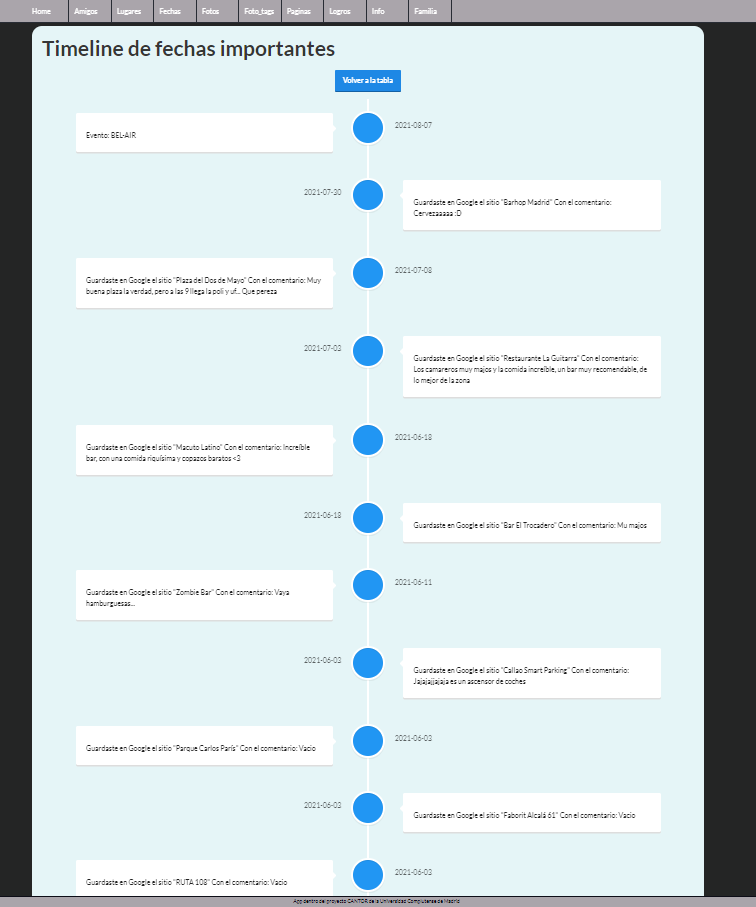
\includegraphics[scale=0.5]{Imagenes/Fuentes/InterfazTimeline.png} \caption{Interfaz de usuario, apartado de timeline}
		\label{WebAplication11}
	\end{center}
\end{figure}
La figura 5.16 muestra las imágenes que nuestra aplicación ha considerado como más importantes para el usuario dentro de Facebook y Google, junto a la descripción que el usuario ha añadido en estas y si han sido fotos de perfil de este o no. En caso de no serlo, ha sido nuestra aplicación la que le ha dado la relevancia.
\begin{figure}
	\begin{center}
		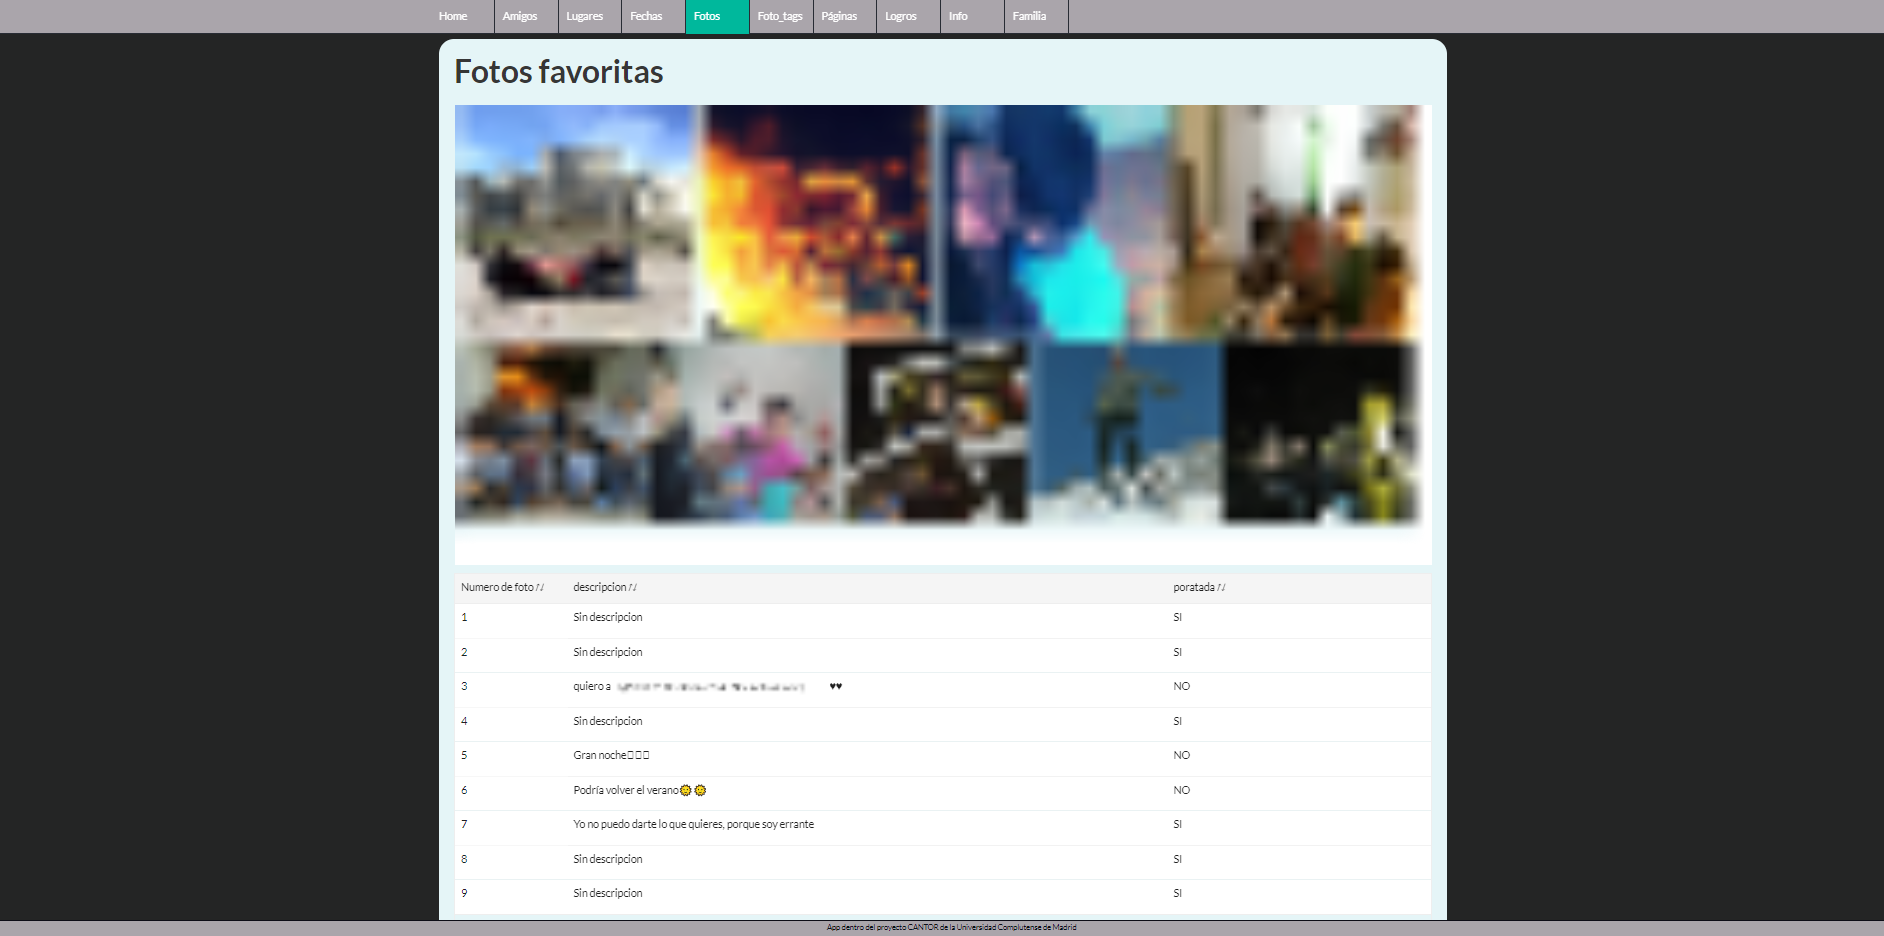
\includegraphics[scale=0.3]{Imagenes/Fuentes/InterfazFotos.png} \caption{Interfaz de usuario, apartado de fotos }
		\label{WebAplication6}
	\end{center}
\end{figure}
La figura 5.17 muestra las galerías de imágenes en las que el paciente ha sido etiquetado con sus mejores amigos, estos se corresponden con los mejores amigos calculados en el anterior apartado de amigos.
\begin{figure}
	\begin{center}
		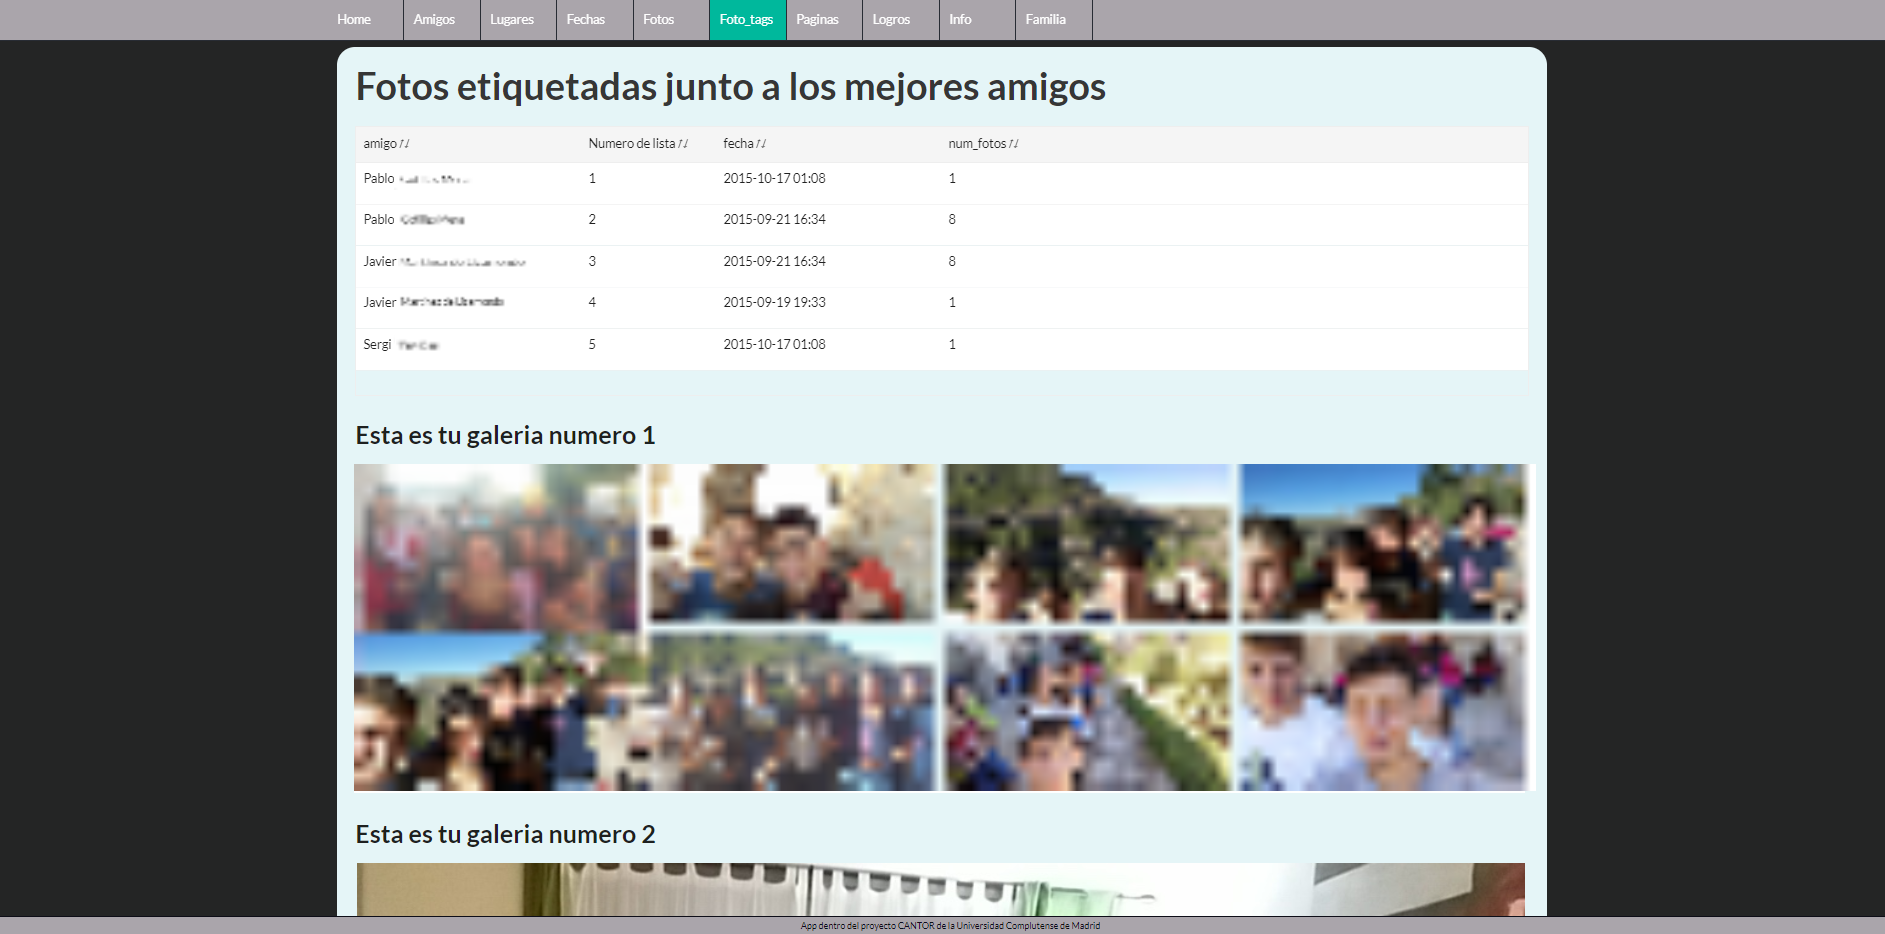
\includegraphics[scale=0.3]{Imagenes/Fuentes/InterfazFoto_tag.png} \caption{Interfaz de usuario, apartado de fotos etiquetadas con amigos}
		\label{WebAplication7}
	\end{center}
\end{figure}
La Figura 5.18 Muestra las páginas con las que el paciente ha interactuado, ordenadas en base a la puntuación que hemos calculado, que indican la relevancia que estas han tenido para el.
\begin{figure}
	\begin{center}
		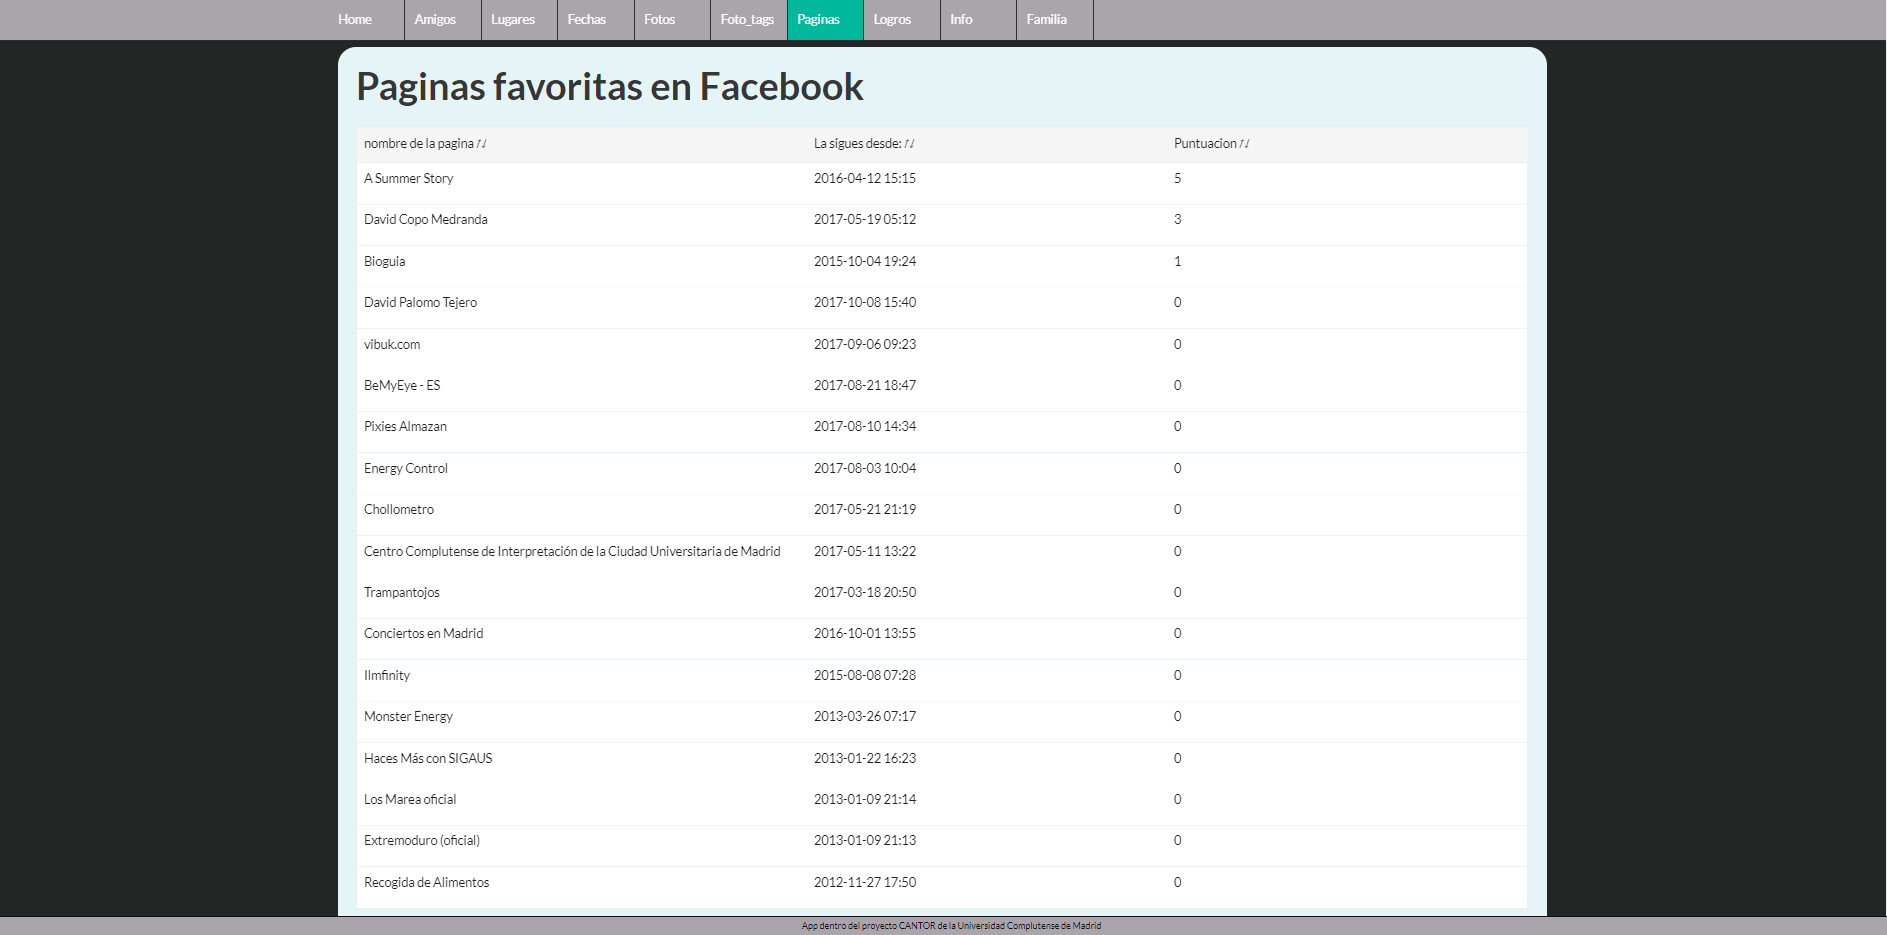
\includegraphics[scale=0.3]{Imagenes/Fuentes/InterfazPaginas.png} \caption{Interfaz de usuario, apartado de páginas favoritas}
		\label{WebAplication8}
	\end{center}
\end{figure}
Las últimas figuras, 5.19 y 5.20 muestran los logros académicos y laborales del paciente y la información personal que el usuario tiene en Facebook, y por último también hay un apartado de familia donde se muestran los familiares que tiene registrados en la misma aplicación.
\begin{figure}
	\begin{center}
		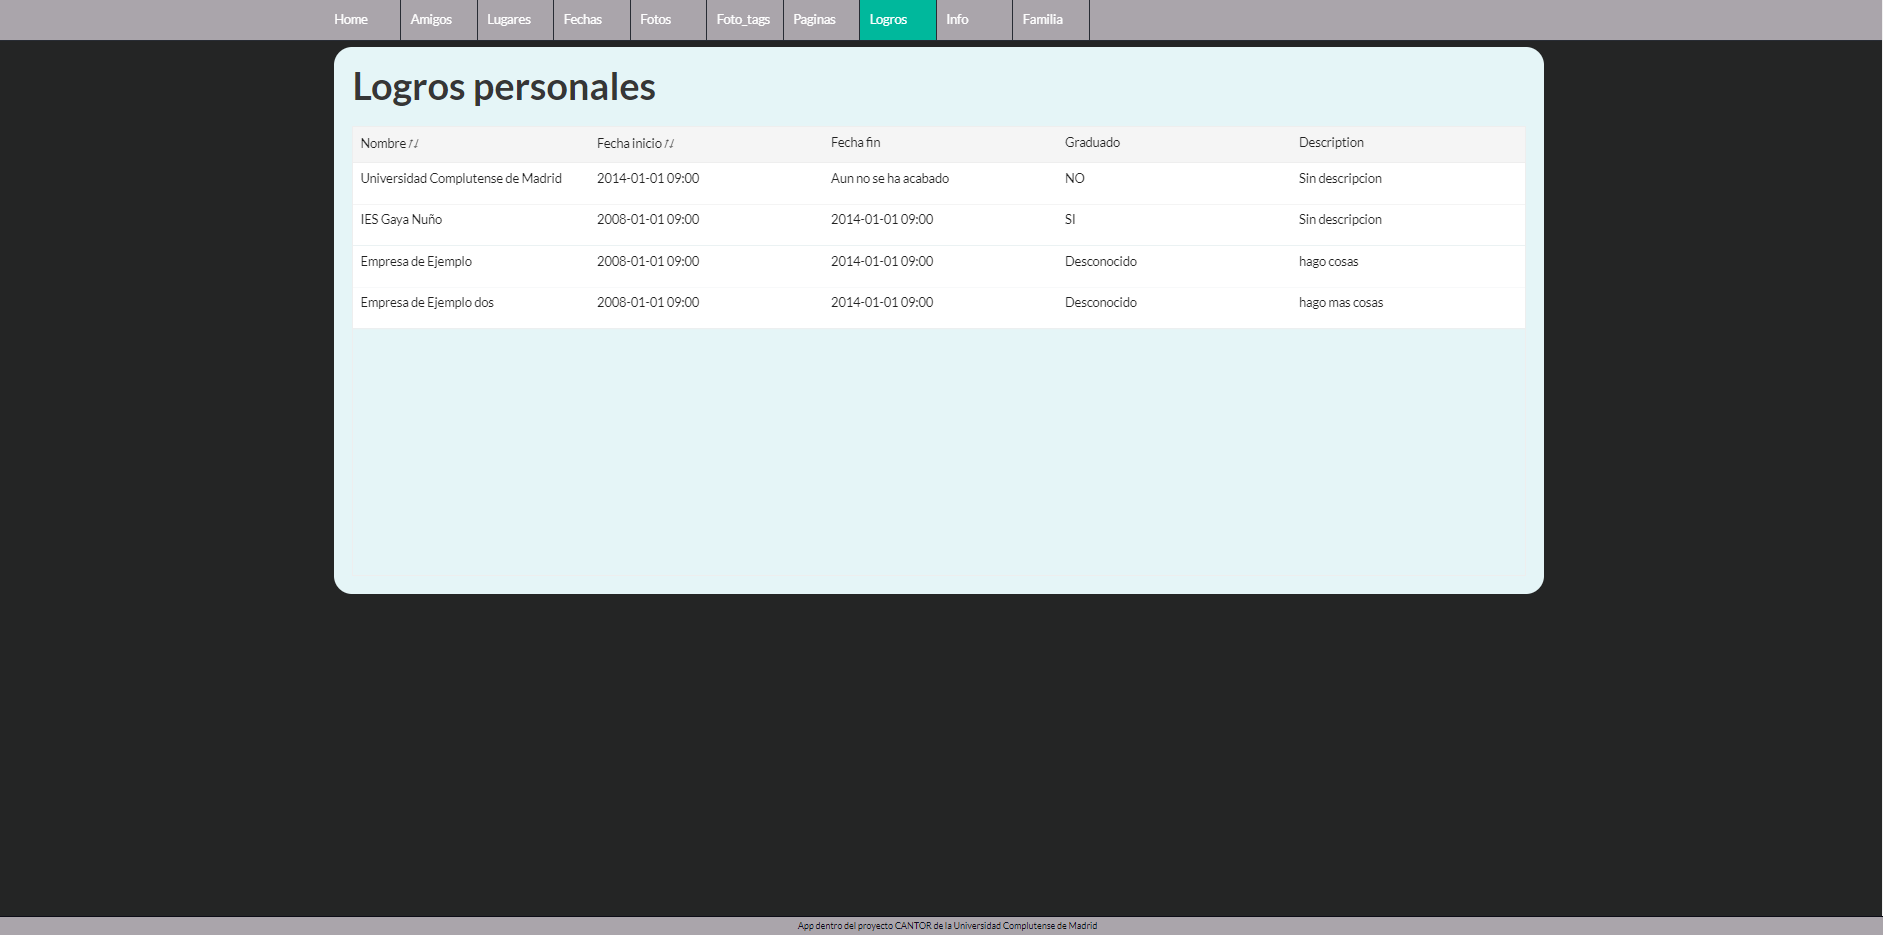
\includegraphics[scale=0.3]{Imagenes/Fuentes/InterfazLogros.png} \caption{Interfaz de usuario, apartado de logros académicos y laborales}
		\label{WebAplication9}
	\end{center}
\end{figure}
\begin{figure}
	\begin{center}
		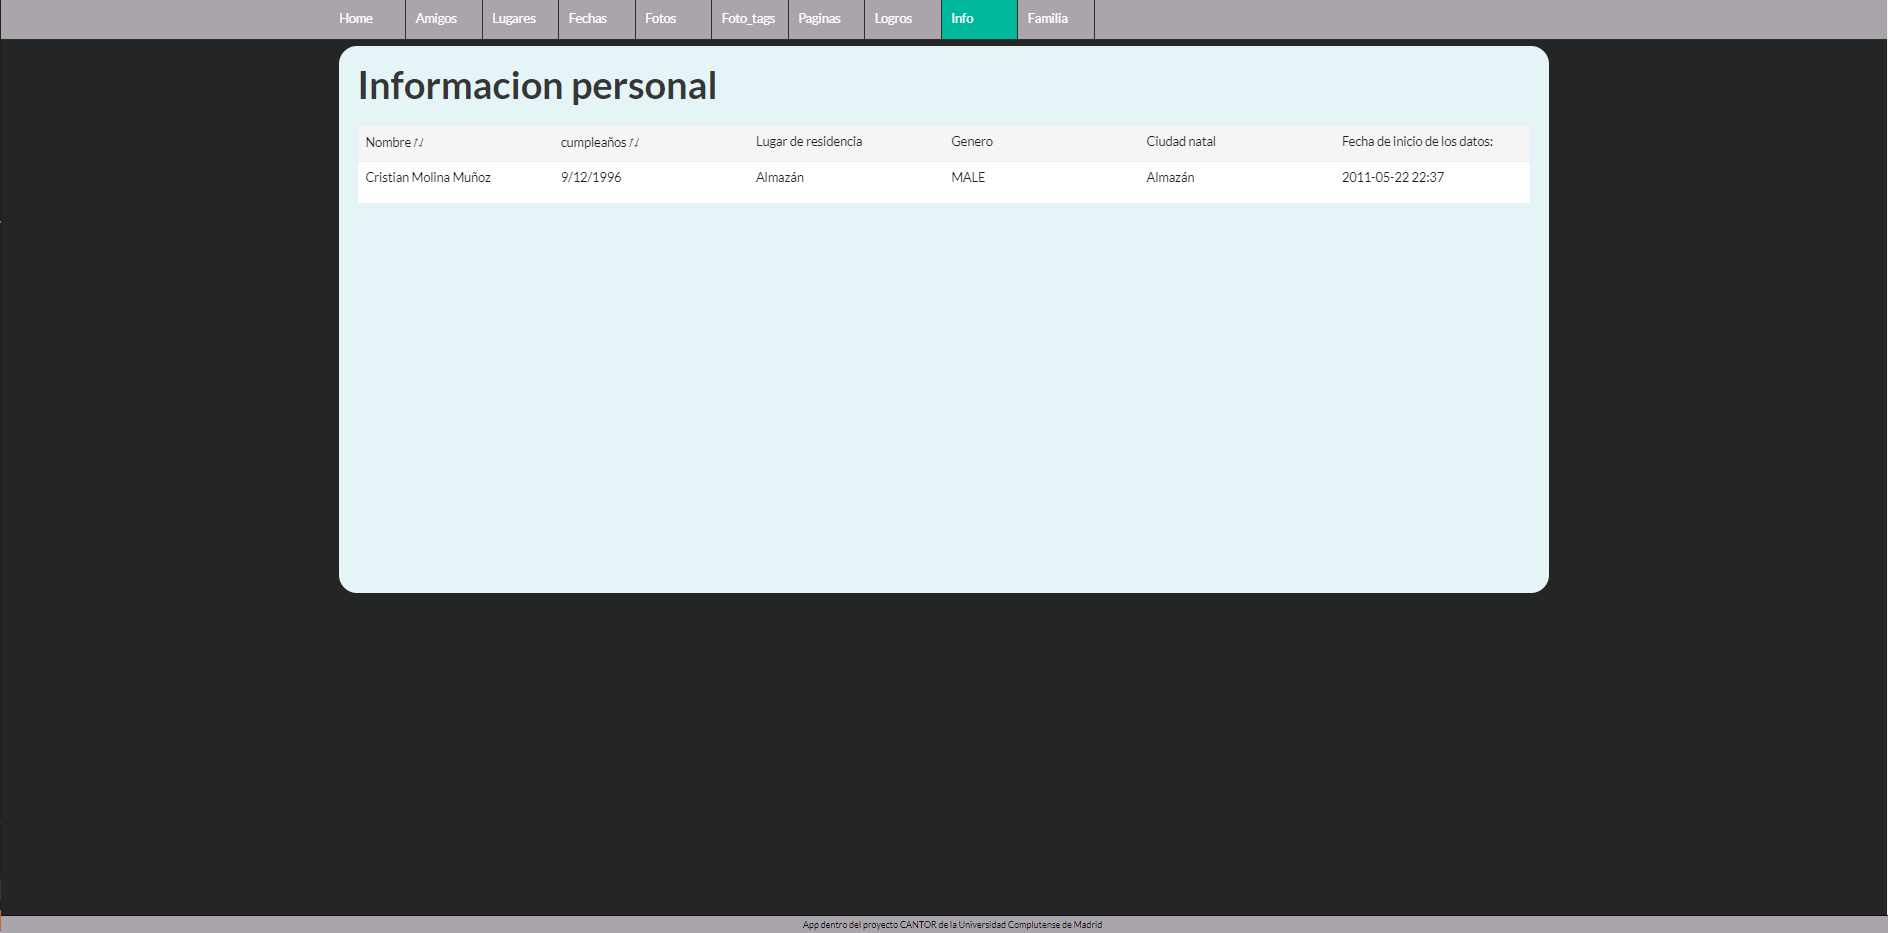
\includegraphics[scale=0.3]{Imagenes/Fuentes/InterfazInfo.png} \caption{Interfaz de usuario, apartado de información personal}
		\label{WebAplication10}
	\end{center}
\end{figure}

Hasta aquí este manual de usuario, esperamos que esta aplicación te sea útil! :D \newpage
